\documentclass[11pt]{amsart}
\usepackage{geometry}                % See geometry.pdf to learn the layout options. There are lots.
\geometry{letterpaper}                   % ... or a4paper or a5paper or ...
%\geometry{landscape}                % Activate for for rotated page geometry
%\usepackage[parfill]{parskip}    % Activate to begin paragraphs with an empty line rather than an indent
\usepackage{graphicx}
\usepackage{amssymb}
\usepackage{epstopdf}
\usepackage[usenames,dvipsnames]{color}
\usepackage{hyperref}
\usepackage{subfig}
\usepackage{float}
\usepackage{dsfont}
\usepackage{wrapfig}
\hypersetup{colorlinks=true}
\DeclareGraphicsRule{.tif}{png}{.png}{`convert #1 `dirname #1`/`basename #1 .tif`.png}
\renewcommand\familydefault{\sfdefault}
\newcommand{\todo}[1]{{\bf\textcolor{red}{TODO: #1}}}
\setlength{\topmargin}{0cm}
\setlength{\headheight}{0cm}
\setlength{\headsep}{1cm}
\setlength{\textheight}{7.7in}
\setlength{\textwidth}{6.5in}
\setlength{\oddsidemargin}{0cm}
\setlength{\evensidemargin}{0cm}
\setlength{\parindent}{0.25cm}
\setlength{\parskip}{0.1cm}

\usepackage{prettyref}
\newrefformat{sec}{Section~\ref{#1}}
\newrefformat{tbl}{Table~\ref{#1}}
\newrefformat{fig}{Figure~\ref{#1}}
\newrefformat{chp}{Chapter~\ref{#1}}
\newrefformat{eqn}{\eqref{#1}}
\newrefformat{set}{\eqref{#1}}
\newrefformat{alg}{Algorithm~\ref{#1}}
\newrefformat{apx}{Appendix~\ref{#1}}
\newcommand\pr[1]{\prettyref{#1}}

\usepackage{fancyhdr,graphicx,lastpage}% http://ctan.org/pkg/{fancyhdr,graphicx,lastpage}
\fancypagestyle{plain}{
  \fancyhf{}% Clear header/footer
  \fancyhead[L]{CSCI-GA.3033-018 - Geometric Modeling}% Right header
  \fancyhead[R]{
\includegraphics[height=20pt]{nyu.pdf}}% Right header
  \fancyfoot[L]{\vspace{2pt} Daniele Panozzo}% Left footer
  \fancyfoot[R]{\vspace{2pt} \thepage}% Right footer
}
\renewcommand{\vec}[1]{\mathbf{#1}}
\newcommand{\bdm}[1]{{\begin{displaymath}#1\end{displaymath}}}
\newcommand{\mtrx}[1] {\begin{bmatrix}#1\end{bmatrix}}
\newcommand{\setR}{\mathds{R}}
\newcommand{\setC}{\mathds{C}}
\newcommand{\itemz}[1]{{\begin{itemize}{#1}\end{itemize}}}

\renewcommand{\vec}[1]{\mathbf{#1}}
\DeclareMathOperator*{\argmin}{argmin}
\def\x{\vec{x}}
\def\c{\vec{c}}
\def\p{\vec{p}}
\providecommand{\abs}[1]{\lvert#1\rvert}
\providecommand{\norm}[1]{\lVert#1\rVert}

\begin{document}

\hspace{50pt}

\begin{center}

{\huge \textbf{Assignment 5: Shape Deformation}}\\
\vspace{10pt}
\end{center}

\section*{Goal of this exercise}
In this exercise, you will implement an algorithm to interactively deform 3D models. You will construct a two-level multi-resolution surface representation and use naive Laplacian editing to deform it.

\section{Multiresolution mesh editing}
For this task, you will compute a mesh deformation based on the rotations and
translations applied interactively to a subset of its vertices via the mouse.
Let $H$ be the set of ``handle'' vertices that the user can manipulate (or
leave fixed). We want to compute a deformation for the remaining vertices,
denoted as $R$.

Let $\mathcal{S}$ be our input surface, represented as a triangle mesh. We want to compute a new surface that contains:
\begin{itemize}
\item the vertices in $H$ translated/rotated using the user-provided transformation $t$, and
\item the vertices in $R$ properly deformed using the algorithm described next.
\end{itemize}

The algorithm is divided in three phases (see Figure \ref{fig:schema}):

\begin{itemize}
\item removing high-frequency details,
\item deforming the smooth mesh, and
\item transferring high-frequency details to the deformed surface.
\end{itemize}

\begin{figure}[h!]
   \centering
   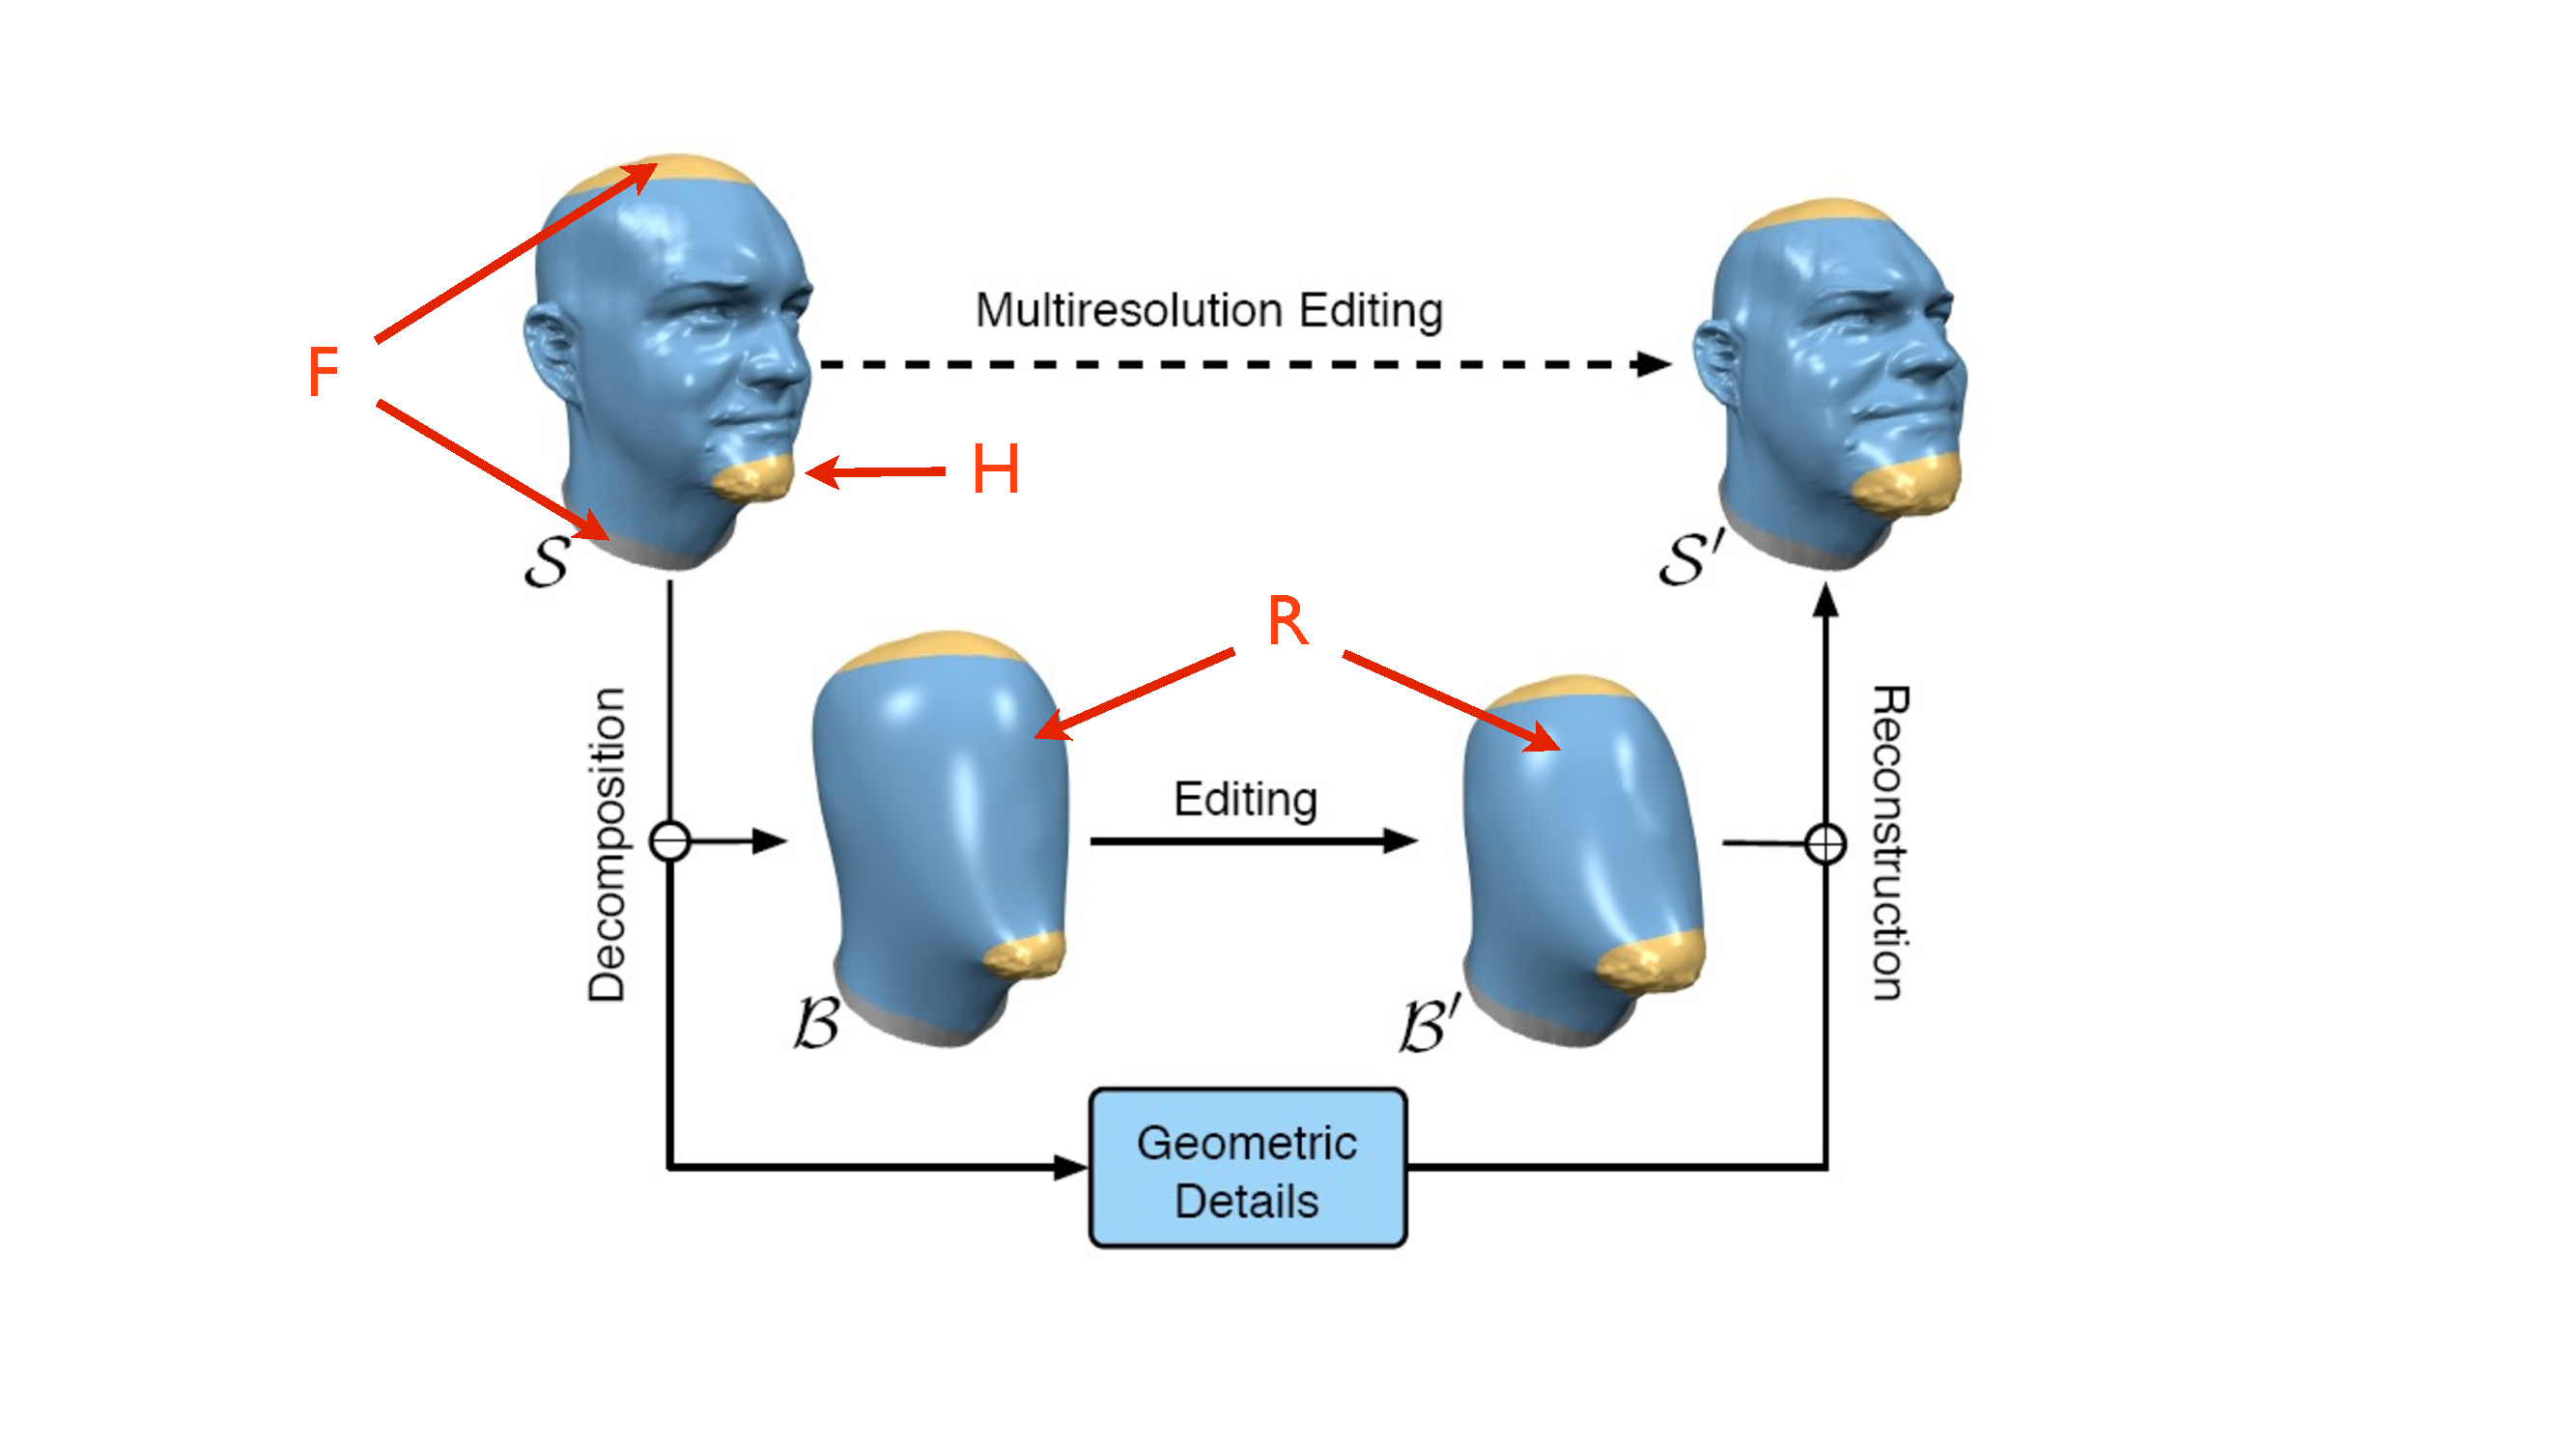
\includegraphics[width=0.7\linewidth]{schema}
   \caption{Algorithm overview}
   \label{fig:schema}
\end{figure}


\subsection{Selecting the handles}
A minimal, lasso-based interface for selecting vertices has been implemented for you. To use it, enable the \texttt{SELECT} mouse mode from the menu (or hit 'S'), click somewhere \textbf{on} the mesh and drag with your mouse to draw a stroke around the area of the mesh you want to select as a handle. The vertices inside the stroked region are saved in the \texttt{selected\_v} variable. You have the options to: (a) accept the selected vertices as a new handle region (only if the vertices are not assigned to a handle already) by hitting the relevant button on the menu or key 'A' (Fig.~\ref{fig:smoothing}(a)), (b) discard the selection and make a new one by drawing another stroke somewhere on the mesh. Once a selection is accepted, you can add additional handles by drawing more strokes.

As selections are accepted, their vertices are saved in the \texttt{handle\_vertices} variable. We also store the handle index for each vertex in \texttt{handle\_id} (-1 if the vertex belongs to no handle). The handle region centroids are stored in \texttt{handle\_centroids}.

The selected handles can be transformed by selecting the appropriate mouse mode (\texttt{TRANSLATE} / \texttt{ROTATE}, shortcuts: ALT+'T', ALT+'R') and dragging with the mouse. While handles are dragged, the updated handle vertex positions are stored in \texttt{handle\_vertex\_positions}.

\subsection{Removal of high-frequency details}

\begin{figure}
   \centering
   \subfloat[\tiny{\emph{hand} mesh.}]{\label{fig:hand}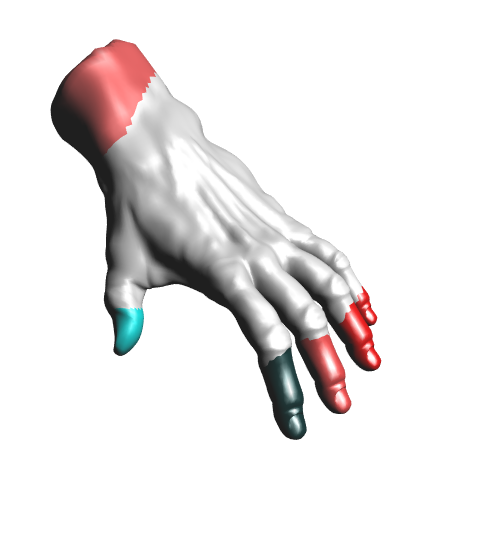
\includegraphics[width=0.23\linewidth]{hand.png}}
%\hspace{0.4cm}
   \subfloat[\tiny{Smoothed \emph{hand}.}]{\label{fig:hand_b}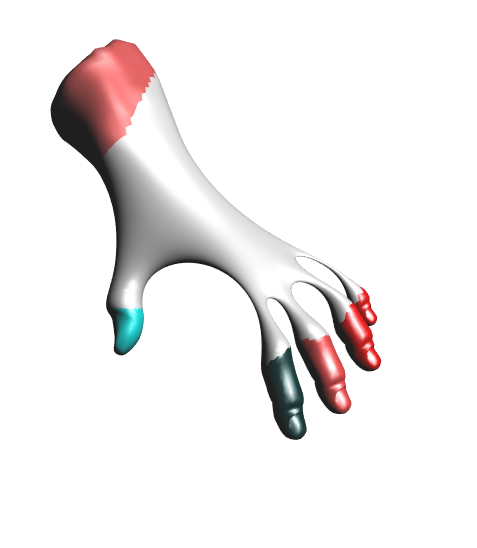
\includegraphics[width=0.23\linewidth]{hand_b.png}}
\hspace{0.5cm}
   \subfloat[\tiny{\emph{woody} mesh.}]{\label{fig:woody}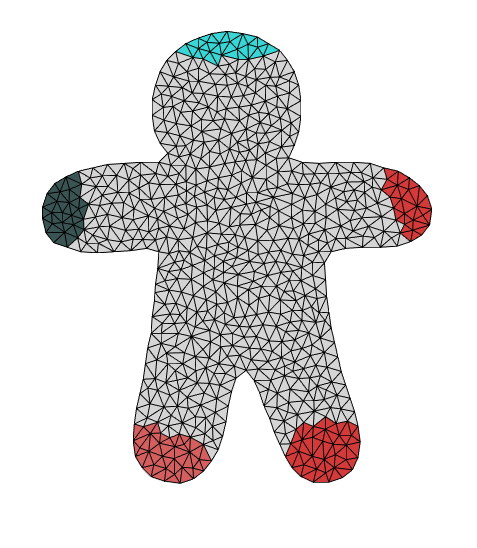
\includegraphics[width=0.23\linewidth]{woody.png}}
%\hspace{0.4cm}
   \subfloat[\tiny{Smoothed \emph{woody}.}]{\label{fig:woody_b}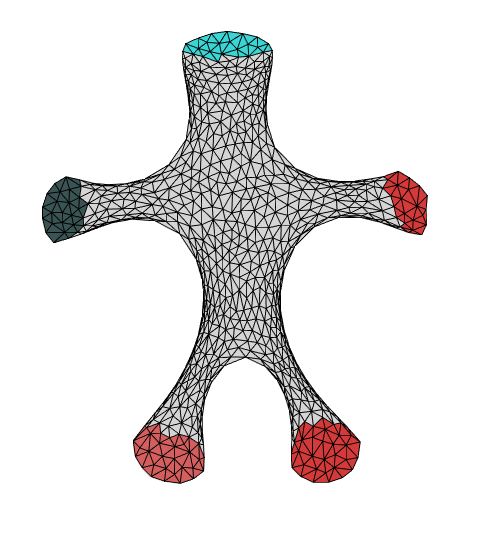
\includegraphics[width=0.23\linewidth]{woody_b.png}}
   \caption{Step 1: Removal of high-frequency details.}
   \label{fig:smoothing}
\end{figure}

We remove the high-frequency details from the vertices $R$ in $\mathcal{S}$ by
minimizing the thin-plate energy, which involves solving a bi-Laplacian system
arising from the quadratic energy minimization:
\begin{eqnarray*} \min_\textbf{v} \textbf{v}^T \textbf{L}_\omega \textbf{M}^{-1} \textbf{L}_\omega \textbf{v} \\
 \mbox{subject to}
 \ \textbf{v}_H = \textbf{o}_H,
\end{eqnarray*}
where $\textbf{o}_H$ are the handle $H$'s vertex positions, $\textbf{L}_\omega$
is the cotan Laplacian of $\mathcal{S}$, and \textbf{M} is the mass matrix of
$\mathcal{S}$.

Notice that $\textbf{L}_\omega$ is the symmetric matrix
consisting of the cotangent weights ONLY (without the division by Voronoi
areas). In other words, it evaluates an ``integrated'' Laplacian rather than an
``averaged'' laplacian when applied to a vector of vertices. The inverse mass
matrix appearing in the formula above then applies the appropriate rescaling
so that the laplacian operator can be applied again (i.e., so that the
Laplacian value computed at each vertex can be interpreted as a piecewise
linear scalar field whose Laplacian can be computed).

%
This optimization will produce a mesh similar to the one in Figure \ref{fig:smoothing}. Note that the part of the surface that we want to deform is now free of high-frequency details.
%
We call this mesh $\mathcal{B}$.

\subsection{Deforming the smooth mesh}
The new deformed mesh is computed similarly to the previous step, by solving the minimization:
\begin{eqnarray*} \min_\textbf{v} \textbf{v}^T \textbf{L}_\omega \textbf{M}^{-1} \textbf{L}_\omega \textbf{v} \\
 \mbox{subject to}
 \ \textbf{v}_H = t(\textbf{o}_H),
\end{eqnarray*}
where $t(\textbf{o}_H)$ are the new handle vertex positions after applying the user's transformation.
We call this mesh $\mathcal{B}'$. See Figure \ref{fig:deform} for an example.

\begin{figure}
   \centering
   \subfloat[\tiny{Deformed/ Smoothed \emph{hand}.}]{\label{fig:hand_t}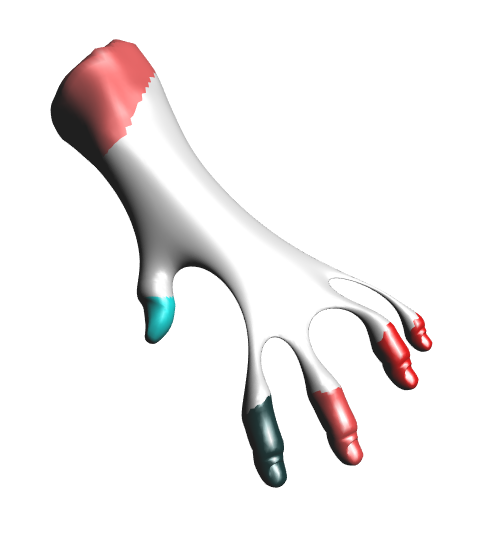
\includegraphics[width=0.23\linewidth]{hand_t.png}}
\hspace{0.9cm}
   \subfloat[\tiny{Deformed/ Smoothed \emph{woody}.}]{\label{fig:woody_t}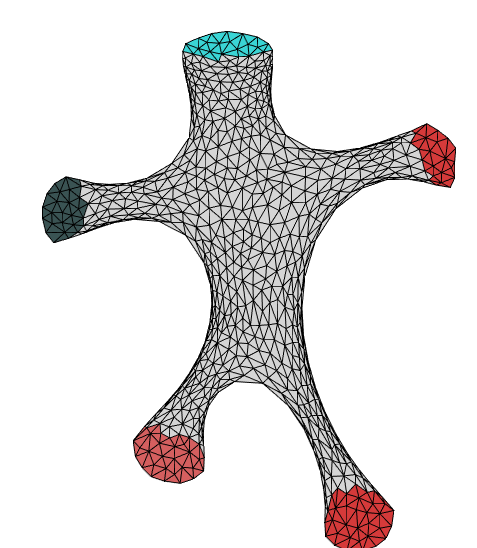
\includegraphics[width=0.23\linewidth]{woody_t.png}}
   \caption{Step 2: Deformation of the smoothed mesh.}
   \label{fig:deform}
\end{figure}

\subsection{Transferring high-frequency details to the deformed surface}
The high-frequency details on the original surface are extracted from $\mathcal{S}$ and transferred to $\mathcal{B}'$. We first encode the high-frequency details of $\mathcal{S}$ as displacements w.r.t. $\mathcal{B}$.

We define an orthogonal reference frame on every vertex $v$ of $\mathcal{B}$ using:
\begin{enumerate}
\item The unit vertex normal
\item The normalized projection of one of $v$'s outgoing edges onto the tangent plane defined by the vertex normal. A stable choice is the edge whose projection onto the tangent plane is longest.
\item The cross-product between (1) and (2)
\end{enumerate}

For every vertex $v$, we compute the displacement vector that takes $v$ from $\mathcal{B}$ to $\mathcal{S}$ and represent it as a vector in $v$'s reference frame.

For every vertex of $\mathcal{B}'$, we also construct a reference frame using the normal and the SAME outgoing edge we selected for $\mathcal{B}$ (not the longest in $\mathcal{B}'$; it is important that the edges used to build both reference frames are the same). We can now use the displacement vector components computed in the previous paragraph to define transferred displacement vectors in the new reference frames of $\mathcal{B}'$. See Figure \ref{fig:displacement} for an example.

Applying the transferred displacements to the vertices of $\mathcal{B}'$ generates the final deformed mesh $\mathcal{S}'$. See Figure \ref{fig:final} for an example.

\begin{figure}[h]
   \centering
   \subfloat[\tiny{Displacements on $\mathcal{B}$ for  \emph{hand}.}]{\label{fig:hand_bd}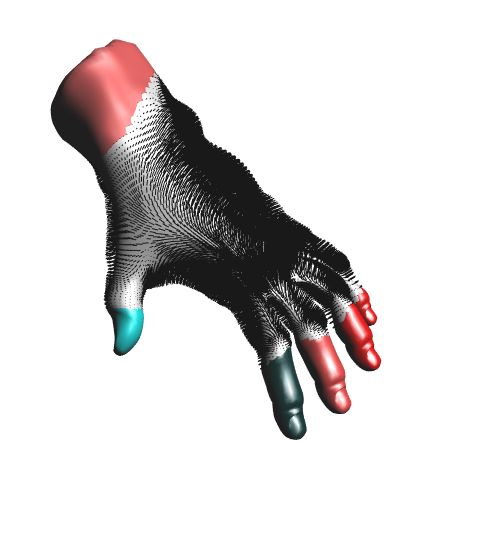
\includegraphics[width=0.24\linewidth]{hand_bd.png}}
%\hspace{0.4cm}
   \subfloat[\tiny{Displacements on $\mathcal{B}'$ for  \emph{hand}.}]{\label{fig:hand_td}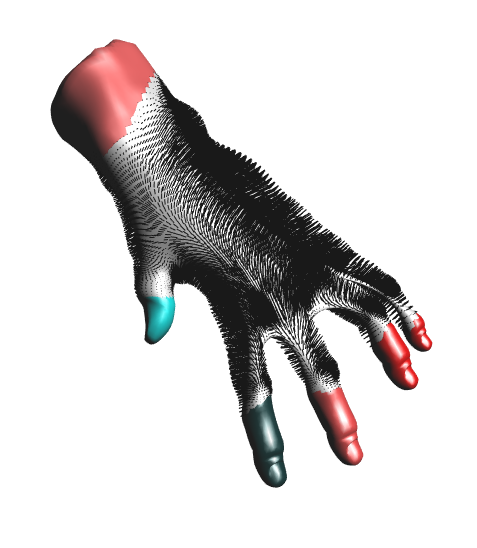
\includegraphics[width=0.24\linewidth]{hand_td.png}}
\hspace{0.5cm}
   \subfloat[\tiny{Displacements on $\mathcal{B}$ for  \emph{woody}.}]{\label{fig:woody_bd}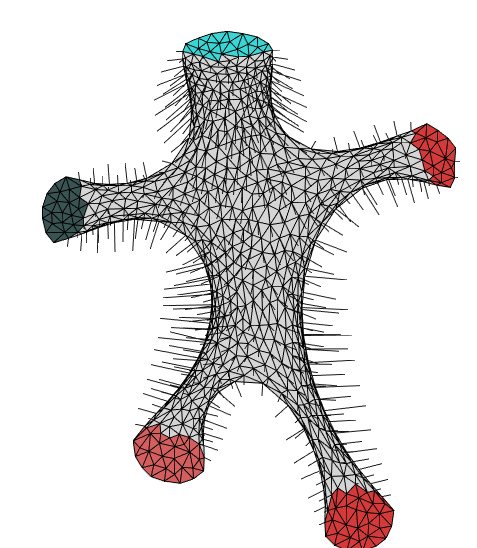
\includegraphics[width=0.24\linewidth]{woody_bd.png}}
%\hspace{0.4cm}
   \subfloat[\tiny{Displacements on $\mathcal{B}'$ for  \emph{woody}.}]{\label{fig:woody_td}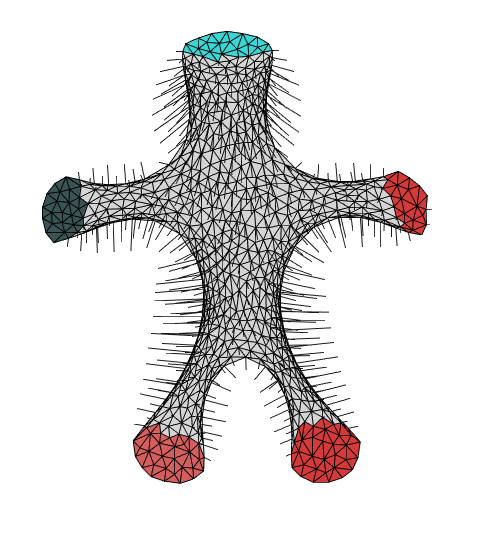
\includegraphics[width=0.24\linewidth]{woody_td.png}}
   \caption{Step 3: Transfer high-frequency details to the deformed surface.}
   \label{fig:displacement}
\end{figure}


\begin{figure}
   \centering
   \subfloat[\tiny{Final \emph{hand} mesh.}]{\label{fig:hand_f}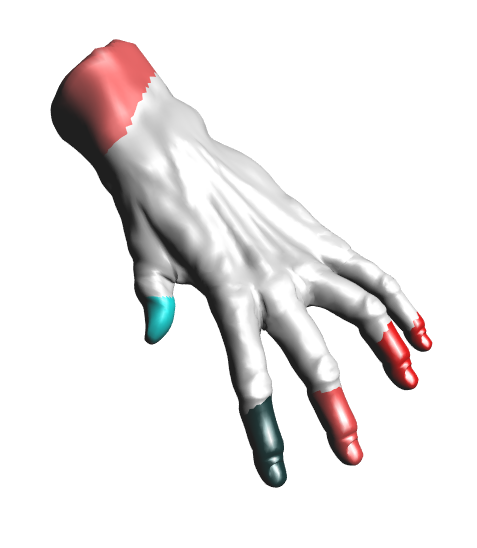
\includegraphics[width=0.23\linewidth]{hand_f.png}}
\hspace{0.9cm}
   \subfloat[\tiny{Final \emph{woody} mesh.}]{\label{fig:woody_f}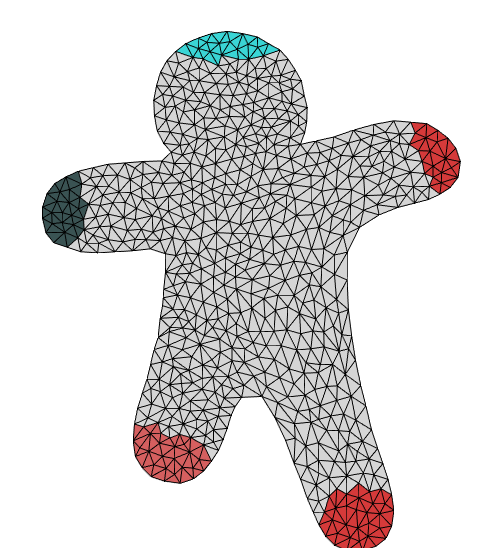
\includegraphics[width=0.23\linewidth]{woody_f.png}}
   \caption{Step 4: Final Deformation Results.}
   \label{fig:final}
\end{figure}

\subsection{Real-time performance}
To achieve real-time performance, you must prefactor the sparse bi-Laplacian matrix appearing in both linear systems. After the user specifies vertex sets $H$ and $F$, you can factorize the matrix $\textbf{L}_\omega \textbf{M}^{-1} \textbf{L}_\omega$ (using a Cholesky ``$LL^T$'' factorization) and then re-use the factorization to solve both linear systems efficiently. This is a mandatory part of the exercise; if your implementation does not achieve interactive frame-rates (10+ fps) on the provided meshes it will not receive the full score.


Required output of this section:
\itemz{
\item{Provide screenshots for 4 different deformed meshes. For each example, provide a rendering of $\mathcal{S}$, $\mathcal{B}$, $\mathcal{B}'$ and $\mathcal{S}'$.}
}

\section{Optional tasks (bonus 5\% )}
\begin{enumerate}
\item
    \emph{(5 points)} Implement the high-frequency detail transfer using ``deformation transfer'', as explained the \href{http://graphics.uni-bielefeld.de/publications/disclaimer.php?dlurl=vmv06.pdf}{paper} \emph{``Deformation Transfer for Detail-Preserving Surface Editing''}, Botsch et al. 2006.
\end{enumerate}

\end{document}
